\input{preamble}
\newcommand{\C}{\mathcal{C}}

\begin{document}

\pagestyle{fancy}
\fancyhead[L]{Seconde}
\fancyhead[C]{\textbf{TD n°4 : fonctions}}
\fancyhead[R]{\today}


\exe{}{
On considère le programme de calcul suivant :
\begin{enumerate}[label=(\roman*)]
\item On prend un nombre entier (positif ou négatif).
\item On divise ce nombre par 3.
\item On ajoute 1 à ce nombre.
\end{enumerate}
Peut-on modéliser ce programme de calcul par une fonction ? Si oui, donner :
\begin{enumerate}
\item Son domaine de définition
\item Sa forme algébrique.
\item L'image du point $1$ par la fonction.
\item Les éventuels antécédent du point $0$ par la fonction.
\end{enumerate}
}{exe:1}{
Appelons $f$ cette fonction.
\begin{enumerate}
\item Le domaine de définition est $\Z$
\item La forme algébrique est $f(x)=\frac{x}3+1$
\item $f(1)=\frac13+1 = \frac43$.
\item On résout $\frac{x}3+1=0$ on trouve $x=-3$.
\end{enumerate}
}

\exe{, difficulty=0}{
	Un étudiant jette une balle dans les airs et mesure la hauteur de la balle tous les quarts de seconde.
	Il note ses résultats dans le tableau ci-dessous.
	\begin{center}
		\def\arraystretch{1.5}
		%\setlength\tabcolsep{20pt}
		\begin{tabular}{|c|c|c|c|c|c|c|c|}\hline
			Hauteur (cm) & 85 & 145 & 190 & 145 & 85 & 40 & 0 \\ \hline
			Temps (s) & 0 & 0,25 & 0,5 & 0,75 & 1 & 1,25 & 1,5 \\\hline
		\end{tabular}
	\end{center}
	
	\begin{enumerate}
		\item La hauteur est-elle une fonction du temps ? Justifier.
		\item Le temps est-il une fonction de la hauteur ? Justifier.
	\end{enumerate}
}{exe:2}{
	\begin{enumerate}
		\item On peut associer \textbf{une seule} hauteur à chaque temps. La hauteur peut donc être vue comme fonction du temps.
		\item On ne peut pas associer un unique temps à chaque hauteur. Par exemple, il y a deux temps distincts pour lesquels la hauteur est de $85$cm (0s et 1s).
		Le temps ne peut donc pas être vu comme fonction de la hauteur.
	\end{enumerate}
}

\exe{}{
On considère la fonction $f$ définie par :
\[ \begin{array}{c c c c}
f : & \R & \to & \R \\
& x & \mapsto & 3x -2
\end{array} \]
\begin{enumerate}
\item Tracer la courbe représentative de $f$ dans un repère orthonormé.
\item Donner le domaine de définition de la fonction $f$. La courbe tracée en 1/ couvre-t-elle tout ce domaine ? 
\item Donner l'image du point $1$ par la fonction $f$.
\item Donner les éventuels antécédent du point $0$ par la fonction $f$.
\end{enumerate}
}{exe:3}{
\begin{enumerate}
\item 
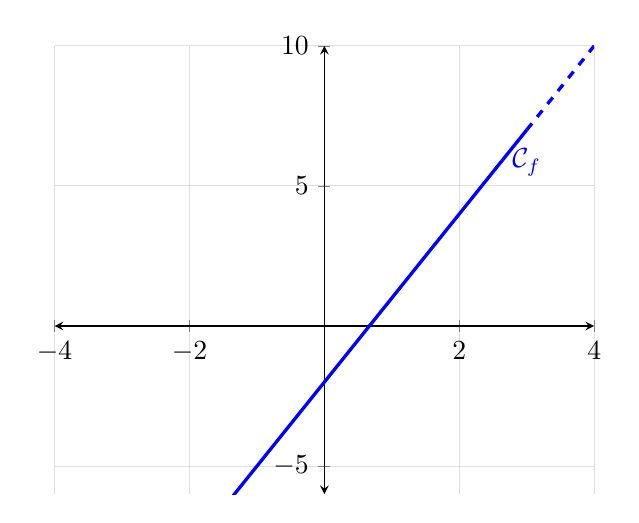
\begin{tikzpicture}[>=stealth, scale=1]
	\begin{axis}[xmin = -4, xmax=4, ymin=-6, ymax=10, axis x line=middle, axis y line=middle, axis line style=<->, xlabel={}, ylabel={}, 		grid=both, grid style = {opacity=.5}]]
		\addplot[blue, very thick, domain =-3:3, samples=2] {3*x-2}  node[below=3pt] {$\C_f$};
		\addplot[blue, very thick, dashed, domain =-4:-3, samples=2] {3*x-2} ;
		\addplot[blue, very thick, dashed, domain =3:4, samples=2] {3*x-2};
	\end{axis}
\end{tikzpicture}
\item $\D_f = \R$, la courbe ne couvre pas tout le domaine car il est infini.
\item $f(1)=1$
\item On résout $3x-2=0$, on trouve $x=\frac23$.
\end{enumerate}
}

\exe{}{
$x$ est une variable réelle.
\begin{enumerate}
\item Traduire l'appartenance de $x$ à chaque intervalle ci-dessous en termes d'inégalités :
\begin{multicols}{2}
\begin{enumerate}
\item $I_1 = ]-3;7[$
\item $I_2 = [4;12]$
\item $I_3 = ]-\infty;0]$
\item $I_4 = [-3;4[$
\end{enumerate}
\end{multicols}
\item En utilisant le résultat de la question précédente, donner une condition pour que $x$ appartienne à l'intervalle $I_1$ \textbf{ET} à l'intervalle $I_4$.
Exprimer ce résultat sous forme d'intervalle.
\end{enumerate}
\textit{Pour deux ensembles quelconques, $A$ et $B$, on note $A \cap B$ leur intersection. \newline
On a $(x \in A$ ET $x \in B) \equi (x \in A \cap B)$}.
}{exe:4}{
\begin{enumerate}
\item
\begin{enumerate}
\item $x \in I_1 \iff -3 < x <7$
\item $x \in I_2 \iff 4 \leq x \leq 12$
\item $x \in I_3 \iff x \leq 0]$
\item $x \in I_4 \iff -3 \leq x < 4$
\end{enumerate}
\item $x \in I_1 \cap I_4 \iff -3 < x < 4$. Autrement dit $I_1 \cap I_4 = ]-3;4[$.
\end{enumerate}
}

\exe{, difficulty=1}{

On considère les fonctions $f$ et $g$ définies par :
\[ \begin{array}{c c c c c c c c c}
f : & \R & \to & \R & \qquad & g : & \R & \to & \R \\
& x & \mapsto & 2x+3 & \qquad & & x & \mapsto & 1-x
\end{array} \]

\begin{enumerate}
\item Tracer une partie des courbes $\C_f$ et $\C_g$ dans un repère orthonormé.
\item Déterminer les images du point $x=0$ par les fonctions $f$ et $g$. Que remarquez-vous ?
\item Déterminer les éventuels antécédents du point $y=0$ par les fonctions $f$ et $g$.
\item Existe-t-il un point $x$ tel que $f(x)=g(x)$. Si oui, le déterminer. Si non, expliquer.
\end{enumerate}

}{exe:5}{
\begin{enumerate}
\item 
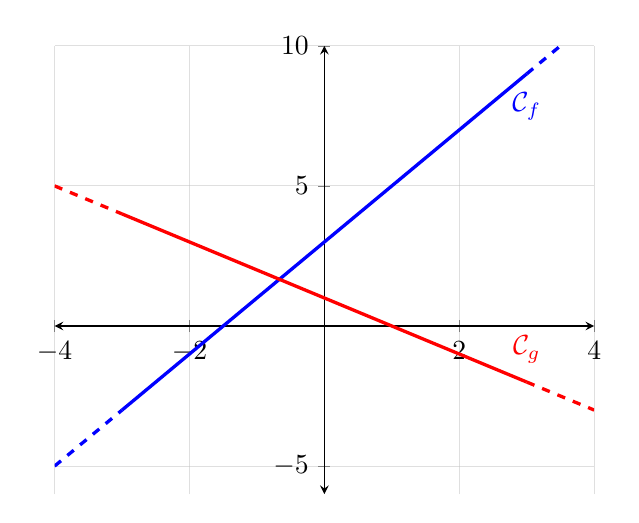
\begin{tikzpicture}[>=stealth, scale=1]
	\begin{axis}[xmin = -4, xmax=4, ymin=-6, ymax=10, axis x line=middle, axis y line=middle, axis line style=<->,
	 xlabel={}, ylabel={}, 		grid=both, grid style = {opacity=.5}]]
		\addplot[blue, very thick, domain =-3:3, samples=2] {2*x+3}  node[below=3pt] {$\C_f$};
		\addplot[blue, very thick, dashed, domain =-4:-3, samples=2] {2*x+3} ;
		\addplot[blue, very thick, dashed, domain =3:4, samples=2] {2*x+3};
		\addplot[red, very thick, domain =-3:3, samples=2] {1-x}  node[above=3pt] {$\C_g$};
		\addplot[red, very thick, dashed, domain =-4:-3, samples=2] {1-x} ;
		\addplot[red, very thick, dashed, domain =3:4, samples=2] {1-x};
	\end{axis}
\end{tikzpicture}
\item $f(0) = 3$ et $g(0) = 1$, on remarque que les images de 0 par les fonctions $f$ et $g$ 
correspondent aux points d'intersection de leurs courbes représentatives avec l'axe des ordonnées.
\item Pour trouver l'antécédent de 0 par $f$ on résout $2x+3=0$ et on trouve $x=-\frac32$. Pour $g$ on trouve $x=1$.
\item On résout $f(x)=g(x)$ et on trouve $x=-\frac23$.
\end{enumerate}
}

\exe{,difficulty=1}{
	Un fonction $f$ admet le tableau de valeurs suivant.
		\begin{center}
		\def\arraystretch{1.2}
		\setlength\tabcolsep{20pt}
		\begin{tabular}{|c|c|c|c|c|}\hline
			$x$ & 0 & -2 & 1 & -1 \\ \hline
			$f(x)$ & 1 & 0 & 0 & 1 \\ \hline
		\end{tabular}
		\end{center}
	Parmis les expressions algébriques suivantes, lesquelles \textbf{ne peuvent pas} correspondre à $f(x)$ ?
		\begin{multicols}{4}
		\begin{enumerate}[label=\roman*)]
			\item $1-x$
			\item $1+\dfrac{x}2$
			\item $\dfrac{1-x}2$
			\item $\dfrac{-x^2 - x + 2}2$
		\end{enumerate}
		\end{multicols}
}{exe:6}{
On remarque que $1-(-2) = 3$ donc i) ne convient pas. De même, $1 + \frac12 = \frac32$ donc ii) ne convient pas.
Enfin $\frac{1-0}2 = \frac12$ donc iii) ne convient pas. En revanche iv) \textbf{pourrait} convenir.
}

\exe{, difficulty=1}{
	Déterminer une fonction numérique $g$, définie sur $\R$ et telle que :
	\[ g(0)=5 \qquad g(3)=0 \]
	Peut-on trouver d'autres fonctions définies sur $\R$ et vérifiant ces deux conditions ? 
}{exe:7}{
On pose $g(x) = ax+b$, la condition g(0)=5 donne $a\times0 + b = 5$  soit $b=5$. 
Ensuite, la condition $g(3)= 0$ donne $3a + 5 = 0$ soit $a=-\frac53$.
Donc la fonction :
\[ \begin{array}{c c c c}
g : & \R & \to & \R \\
& x & \mapsto & -\frac53x + 5
\end{array} \]
convient.
On peut trouver d'autres fonctions vérifiant ces conditions, il suffit pour cela de considérer la fonction :
\[ \begin{array}{c c c c}
h : & \R & \to & \R \\
& x & \mapsto & x(x-3)
\end{array} \]
Comme $h(0)=0$ et $h(3)=0$, pour tout réel $k$ la fonction définie par :
\[ \begin{array}{c c c c}
f : & \R & \to & \R \\
& x & \mapsto & g(x) + k \times h(x)
\end{array} \]
convient. On a donc donné une infinité de solutions.
}

\exe{, difficulty=2}{
On rappelle la formule de double distributivité, soient $a, b, c$ et $d$ quatre nombres réels quelconques. On a :
\[ (a+b)(c+d) = ac + ad + bc + bd . \]
En particulier, si $a=c$ et $b=d$, on obtient l'identité remarquable :
\[ (a+b)^2 = a^2 + 2ab + b^2. \]
Ces formules sont à connaître \textbf{par coeur}. \newline
\begin{enumerate}
\item Donner une expression développée de $(a-b)^2$. \newline
\textit{Indication : remplacer $b$ par $-b$}.
\item On considère la fonction :
\[ \begin{array}{c c c c}
f : & \R & \mapsto & \R \\
& x & \to & x^2 - 4x +10
\end{array} \]
Démontrer que $f(x)=6+(x-2)^2$.
\item En conclure que, pour tout $x \in \R, f(x) \geq 6$.
\item Donner un nombre $x_0 \in \R$ tel que $f(x_0)=6$.
\end{enumerate}
}{exe:8}{
Exercice de recherche.
}

%\exe{, difficulty=2}{
%
%}{exe:9}{
%
%}

%%%%%%%%%%%%

\newpage
\fancyhead[C]{\textbf{Solutions}}
\shipoutAnswer



\end{document}
